\newpage
\changeindent{0cm}
\section{提案手法}
\changeindent{2cm}

本章では,本研究の提案手法について説明する.

\changeindent{0cm}
\subsection{漫画のセリフのマルチモーダルな感情推定手法}
\changeindent{2cm}

本研究では, 4 コマ漫画ストーリーデータセットを用いて,
各セリフにアノテートされた感情ラベルを推定するタスクを解き, その精度を確認する.

図 \ref{fig:teian} にマルチモーダルな推定手法として, 提案手法の概要を示す.
図 \ref{fig:teian} のように, ある 4コマ漫画の中の 1 コマがあって, このコマに含まれている ``キャー!" というセリフのラベルを推定することを例に取って説明する.

自然言語処理のみを用いた推定を行う場合は, Text Embedding 層の入力として適した形式にこのセリフを整形し, 出力として得たセリフの分散表現 (以下, ``セリフベクトル" と呼ぶ) を識別器への入力とすることで対応する感情ラベルを推定する. そして, マルチモーダルな推定を行う場合は, このセリフが含まれているコマ画像全体を Image Embedding 層への入力とし, 得られたコマ画像の分散表現 (以下, ``コマベクトル" と呼ぶ) をセリフベクトルと結合させたベクトルを識別器への入力とすることで対応する感情ラベルを推定する.

\begin{figure}[h]
  \centering
  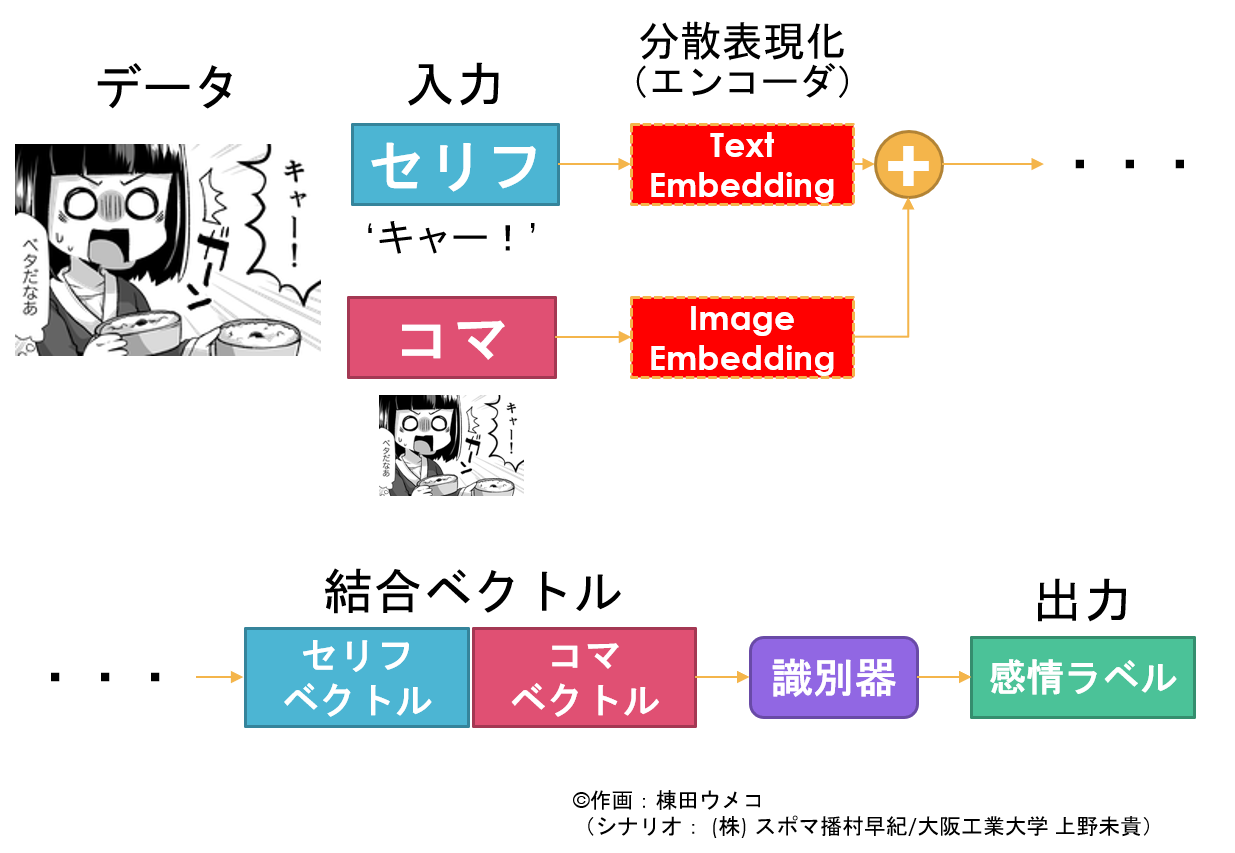
\includegraphics[width=0.7\hsize]{doc/figures/teian_2.png}
  \caption{提案手法の概要}
  \label{fig:teian}
\end{figure}

\newpage
\changeindent{0cm}
\subsection{シソーラスを用いたデータ拡張}
\changeindent{2cm}

4 コマ漫画ストーリーデータセットの問題点として, データ数が少ないことがあげられる.
そこで, 本研究では日本語 WordNet \cite{word_net_jp} のシソーラスを用いてテキストデータを拡張する.

図 \ref{fig:data_aug} にシソーラスを用いたデータ拡張の概要を示す.
分かち書きされたオリジナルのセリフに対して, 日本語 WordNet で類似語を持つ単語について類似語に置き換え, 文を生成することでテキストデータを拡張する. ただし, 文の中に類義語を持つ単語が
複数あった場合, 類似語に置き換える単語は同時に 1 つまでとし, 英数字・記号のみで表されている類似語は除外する. 例えば, 5 つの単語からなる文章があり,
各単語が 5 つの類似語を持っている場合, その文からは新しく 25 文が生成されることとなる.

\begin{figure}[h]
  \centering
  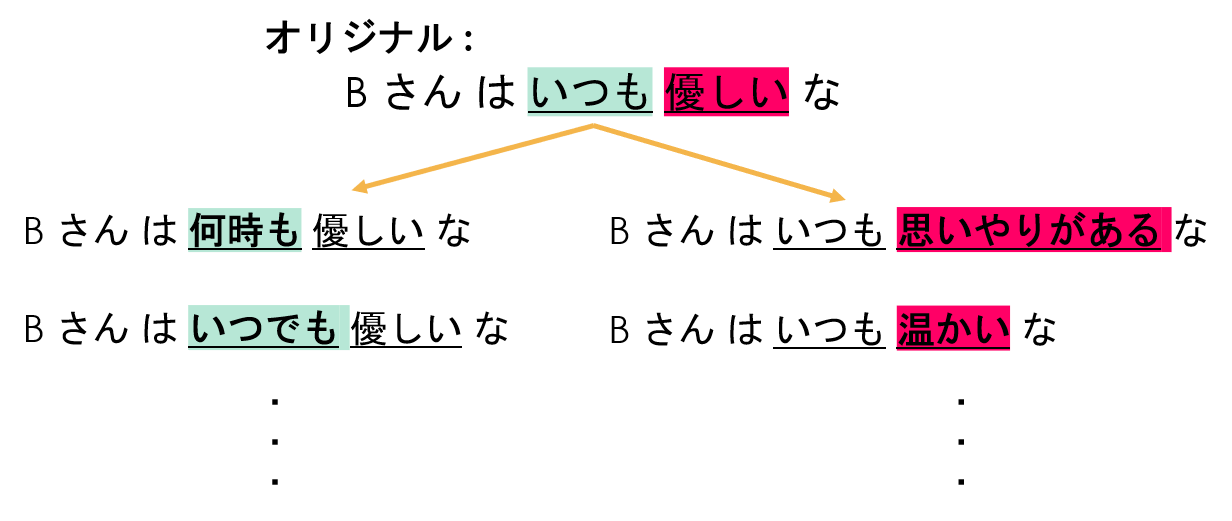
\includegraphics[width=0.8\hsize]{doc/figures/data_aug.png}
  \caption{シソーラスを用いたデータ拡張の概要}
  \label{fig:data_aug}
\end{figure}
